\section{Optimizing the Shipped Recipe}
\label{sec:extended}

The two-path harness of Section~\ref{sec:eval} deliberately excludes optimizations that would apply to only one path. This section adds them to form the shipped configuration and measures each step at Netflix $K=96$, where all of them are active.
\subsection{Weighted Regularization}
\label{ssec:weightedlambda}

An early version of this work used a uniform penalty $\lambda I$ with $\lambda = 0.1$. Under it, heavily rated entities are under-regularized as $K$ grows, and the Netflix test RMSE of both paths rose from $0.8607$ at $K=16$ to $1.1929$ at $K=96$. The weighted penalty $\lambda n_u I$ of \eqref{eq:als_update} removes this effect, and test RMSE then falls monotonically ($0.8311$, $0.8233$, $0.8205$, $0.8191$, $0.8176$ for $K = 16$ to 96). Entities without training ratings keep the uniform term to stay positive definite.

The coefficient was selected by a sweep of eight values from $0.010$ to $0.120$ at $K=96$. Both Netflix and ML-20M show a U-shaped error curve with the minimum in $[0.040, 0.048]$ (Supplementary Table~S2). The value $\lambda = 0.048$, used for every result in this paper, is the ML-20M optimum. It is not optimal for Netflix: $\lambda = 0.040$ lowers the Netflix test RMSE by $0.35\%$ ($0.8142$ versus $0.8171$, both with momentum) and would cost ML-20M $0.23\%$.
\subsection{Narrower-Precision Solver at $K=96$}
\label{ssec:fp16solver}

At $K=96$ the blocked solver is limited by shared-memory capacity (23.1~KB per block). Storing the $K \times K$ factor tiles in FP16, while keeping the right-hand side, diagonal inverses, and all arithmetic in FP32, halves that footprint. Under the uniform penalty this variant is unusable, because heavily rated entities have condition numbers in the hundreds of thousands. Under the weighted penalty the condition number is $O(K/\lambda)$, and the FP16-tile solver reproduces the FP32 solver's test RMSE exactly (Netflix $K=96$: $0.817558$ for both), with no non-finite solves detected by an in-kernel guard. It reduces the solve stage by $23\%$ and total training time from $10.59$~s to $9.44$~s. At $K \le 64$ it is not used: the diagonal entries of the most-rated items sum over up to 187{,}512 ratings and, with larger factor components at lower rank, overflow FP16 ($4{,}571$ failed solves at $K=32$, 61 at $K=64$, none at $K=96$). With $\kappa$ the condition number of the regularized system, the worst-case bound gives $\kappa\,\varepsilon_{16} \approx 1$ at $K=96$, although typical systems are far better conditioned, so this result is a single measurement, not a general guarantee.

\subsection{Removing Non-Solver Overheads}
\label{ssec:nonsolver}

With the FP16-tile solver in place, an Nsight Systems timeline at $K=96$ shows two non-arithmetic phases taking about a fifth of GPU time: the periodic RMSE check ($16\%$) and a separate pass that adds $\lambda n_u$ to each diagonal ($6\%$). We fused the diagonal update into the solver's load phase, bit-identically. For $K \ge 32$ we replaced the RMSE kernel with a warp-per-entity version that walks the ratings in compressed sparse row (CSR) order and reads the FP16 factor copies already maintained for the tensor cores; the final reported RMSE is still computed in FP32. On Netflix at every rank, runs with and without the fast check stop at the same sweep with bit-identical test RMSE. We also rewrote the giant-tier kernel to stage its loads with asynchronous copies. Measured in the shipped binary, these changes together reduce the Netflix $K=96$ time from $9.35$~s to $7.75$~s ($1.21\times$) with unchanged RMSE. A vendor batched factorization ($2.8\times$ slower than our solver) and a tensor-core formulation of the solve (2.1--2.3~TFLOP/s, launch-bound) were tried and discarded.

\subsection{Momentum Acceleration}
\label{ssec:momentum}

The optimizations above shorten each sweep; momentum reduces the number of sweeps. Near its solution, ALS behaves as a contractive fixed-point iteration, so its factor sequence can be extrapolated with a heavy-ball step: after each solve, $X \leftarrow X_{\text{new}} + \beta (X_{\text{new}} - X_{\text{prev}})$, and likewise for $Y$. The extrapolation term vanishes at a fixed point, so any limit of the extrapolated iteration is a fixed point of ALS; convergence itself is checked empirically. Its cost is negligible, and $\beta = 0.3$ is used for every dataset and rank. Larger values fail: $\beta = 0.4$ oscillates enough to cancel the savings, and $\beta = 0.5$ makes the factors large enough to overflow the FP16 solver tiles. An in-kernel guard found no non-finite solves at $\beta = 0.3$.

\begin{table}[!t]
\caption{Effect of Momentum ($\beta=0.3$), RTX 3060. All Runs Converge in 15 Sweeps (Without Momentum: 20 on Netflix, 25 on MovieLens). $\Delta$RMSE Is the Change in Test RMSE in Units of $10^{-4}$ (Negative Is Better). ``Total'' Is the End-to-End Speedup of the Shipped Recipe over the FP32 Baseline of Table~\ref{tab:main3060}}
\label{tab:momentum}
\centering
\footnotesize
\renewcommand{\arraystretch}{1.02}
\setlength{\tabcolsep}{4pt}
\begin{tabular}{llrrrrr}
\toprule
\textbf{Dataset} & & \textbf{$K{=}16$} & \textbf{32} & \textbf{48} & \textbf{64} & \textbf{96} \\
\midrule
\multirow{2}{*}{Netflix}
 & $\Delta$RMSE   & $+0.4$ & $-1.7$ & $-3.4$ & $-4.3$ & $-4.1$ \\
 & total          & 5.6$\times$ & 10.1$\times$ & 15.3$\times$ & 21.0$\times$ & \textbf{26.0$\times$} \\
\midrule
\multirow{2}{*}{ML-32M}
 & $\Delta$RMSE   & $-3.9$ & $-4.0$ & $-4.9$ & $-5.3$ & $-4.8$ \\
 & total          & 7.7$\times$ & 11.4$\times$ & 15.9$\times$ & 20.2$\times$ & 21.7$\times$ \\
\midrule
\multirow{2}{*}{ML-20M}
 & $\Delta$RMSE   & $-1.6$ & $-3.7$ & $-5.5$ & $-5.5$ & $-5.4$ \\
 & total          & 7.1$\times$ & 11.1$\times$ & 15.6$\times$ & 20.4$\times$ & 23.2$\times$ \\
\midrule
\multirow{2}{*}{ML-10M}
 & $\Delta$RMSE   & $-0.9$ & $-4.3$ & $-5.8$ & $-5.7$ & $-5.6$ \\
 & total          & 6.7$\times$ & 10.4$\times$ & 14.4$\times$ & 19.1$\times$ & 22.2$\times$ \\
\bottomrule
\end{tabular}
\end{table}

Momentum cuts wall time by $1.30$--$1.33\times$ on Netflix and $1.62$--$1.66\times$ on MovieLens (Table~\ref{tab:momentum}). Test RMSE is equal or better at 19 of the 20 points. The exception is Netflix $K=16$, where it rises by $4.2 \times 10^{-5}$ ($0.831057$ to $0.831099$); five repeated runs confirm this small loss.

\subsection{Cumulative Ablation}
\label{ssec:ablation}

Fig.~\ref{fig:ablation} combines the steps at Netflix $K=96$. The first four bars come from the two-path harness and the last two from the shipped binary, which runs the configuration of the fourth bar in $9.35$~s. The third bar is the FP32-solver reference against which the solver change was measured. It comes from an earlier build of the harness and is $1.7\%$ slower than the second bar, a difference between builds rather than an optimization. The tensor-core dispatch is by far the largest factor ($14.8\times$). The FP16-tile solver and overhead removal together add $1.34\times$ (from $10.41$~s to $7.75$~s), and momentum adds $1.31\times$. Momentum does not depend on precision, so an FP32 baseline could also benefit from it; if the baseline is given the same 15-sweep count, the advantage of the shipped recipe is $19.5\times$ rather than $26.0\times$. We therefore report $14.8\times$ as the effect of the precision dispatch, $19.5\times$ as the iteration-matched advantage, and $26.0\times$ as the end-to-end speedup of the shipped recipe.

\begin{figure}[!t]
\centering
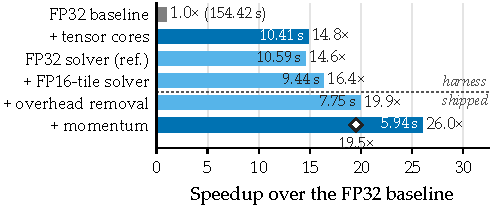
\includegraphics[width=\columnwidth]{figures/fig_ablation.pdf}
\caption{Cumulative ablation at Netflix $K=96$ on the RTX~3060, with wall time inside each bar. Bars above the dashed line come from the two-path harness, and bars below from the shipped binary. The fourth bar takes $9.44$~s in the harness and $9.35$~s in the shipped binary. The steps follow Sections~\ref{ssec:fp16solver}--\ref{ssec:momentum} in order (overhead removal: fused $\lambda$, fast RMSE check, asynchronous giant-tier copies). The diamond marks $19.5\times$, the advantage if the baseline also stops at 15 sweeps.}
\label{fig:ablation}
\end{figure}
